\chapter{Background}
\section{Natural Language Processing}
Natural language processing (NLP) is a subfield of linguistics, computer science, information engineering, and artificial intelligence concerned with the interactions between computers and human (natural) languages, in particular how to program computers to process and analyze large amounts of natural language data \cite{nlpdefinition}.

\subsection{NLP Pipeline}
Typical NLP pipelines consist of multiple parts all of which add value to the output and are crucial for any advanced tasks performed on text. Common tasks include tokenization, part of speech tagging, stemming and others.

\begin{figure}[H]
\begin{center}
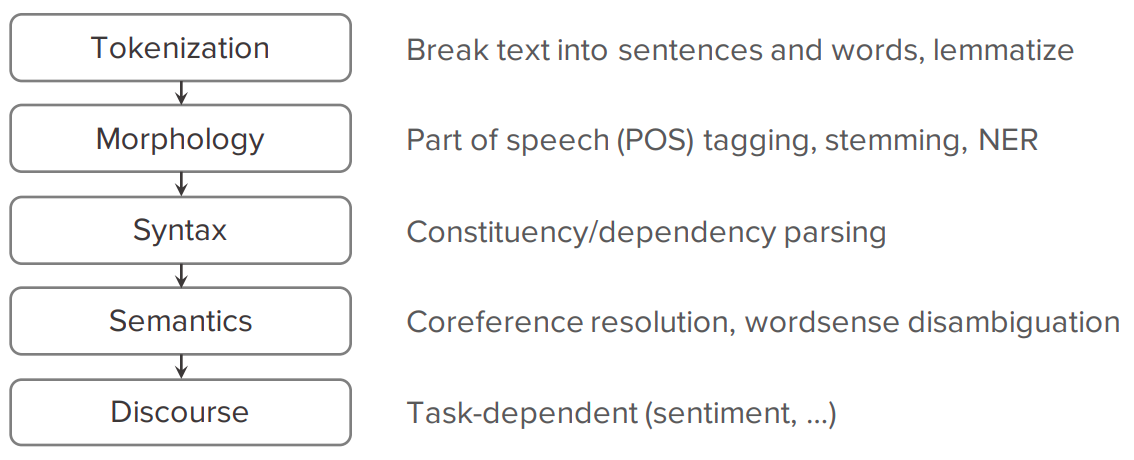
\includegraphics[scale=0.3]{classicalnlppipeline.png}
\caption{Typical NLP pipeline \cite{nlppipeline}}
\end{center}
\end{figure}

\subsubsection{Stopword Removal}
Stopword removal is a common data cleaning technique. Stopwords are common words, which do not provide a lot of value at tackling the task. For example, words such as \textit{and, for, but, on}. Stopwords can be context dependent. Removing stopwords reduces dataset size and lowers the amount of noise in the data, thus improving performance and accuracy of the other pipeline components.

\subsection{Information Retrieval}
Information retrieval is focused on finding documents relevant to the query. While its traditional use cases revolve around search engines it can also be used in other tasks, such as classification. Information retrieval methods are most often based on terms, which can be words or n-grams.

\subsubsection{N-grams}
N-gram is a contiguous sequence of \textit{n} items from a given sample of text or speech \cite{ngramwiki}. The items can be phonemes, syllables, letters or words \cite{ngramwiki}. In this project only word n-grams are going to be used.

\subsubsection{Term Frequency (TF)}
Term frequency assigns weights to words in a set of documents, and it is a count of all of the occurences of a term in a document or a whole dataset. While it is not an accurate weighting method, using it on whole dataset together with n-grams has a potential of providing useful insights into the dataset.
\subsubsection{Inverse Document Frequency (IDF)}
Inverse document frequency is another term weighting method. Document frequency for term \textit{t} shows in how many documents does the term appear. However, it is evident that the most informative and discriminative terms are the ones which occurs in less documents rather than all of them. For example, "spider" is a much more helpful query term than "and". Therefore, inversed document frequency is used.

It is calculated by dividing a total number of documents (\textit{N}) by the number of documents that contain the term (\textit{$df_{t}$}) and then applying the logarithm. The resulting formula is:
\[ idf_{t} = log_{10}(N/df_{t}) \]

\subsubsection{Term Frequency - Inverse Document Frequency (TF-IDF)}
Term Frequency - Inverse Document Frequency (TF-IDF) is very well known and widely used in information retrieval. It is calculated by multiplying term frequency of a term in a specific document ($TF_{i, j}$) with an inverse document frequency of a term in the dataset ($IDF_{i}$):
\[ w_{i,j} = tf_{i,j} * log_{10}(N/df_{t}) \]

\subsubsection{Cosine Similarity}
Cosine similarity is a measure of similarity between vectors, which is often usedn technique in information retrieval. Using cosine similarity it is possible to find documents or sentences that are most similar to the given query. For length-normalized vectors, cosine similarity is a dot product:
\[cos(\vec{a},\vec{b})=\vec{a} \cdot \vec{b}\]
\subsection{Word Embeddings}
Word embeddings are mappings of words or phrases of the vocabulary to vectors of real numbers. One of the biggest breakthroughs in word embeddings has been in 2013 with the creation of Word2vec by Google \cite{wordembeddingwiki}. Since then there have been created a few even more advanced models such as BERT, ELMo and ULMfit, which are contextualixed word embedding models (also called language models) \cite{languagemodels} and are a current state-of-the-art.

One of the core advantages of word embeddings are that they can also be pre-trained on a specific dataset, this way improving their performance in the specific context or in specific tasks.
\subsection{Topic Modelling Using LDA}
\label{sec:lda}
Topic modelling is a procedure of extracting topics from documents. There are multiple multiple topic modelling methods available, but one of the most popular ones is latent Dirichlet allocation (LDA).

LDA is an unsupervised machine learning algorithm, as it does not use labeled data, but generates topics based on statistics \cite{ldawiki}. LDA treats every document as a bag-of-words (i.e. order does not matter) and the key assumption is that the way the document was generated was by picking a set of topics and then for each topic a set of words \cite{ldaexplanation}. And then it basically reverse engineers the process by the following algorithm:
\begin{enumerate}
\item Assume there are \textit{k} topics across the all of the provided documents.
\item Distribute these \textit{k} topics across document \textit{m} (this distribution is known as $\alpha$) by assigning each word a topic.
\item For each word \textit{w} in document \textit{m}, assume its topic is wrong but every other word is assigned the correct topic.
\item Probabilistically assign word \textit{w} a topic based on what topics are in document \textit{m} and how many times word \textit{w} has been assigned a particular topic across all of the documents (this distribution is called $\beta$).
\end{enumerate}

\begin{figure}[H]
\begin{center}
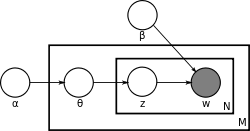
\includegraphics[scale=1.3]{LDAplate.png}
\caption{LDA model plate diagram \cite{riskpaper1}}
\end{center}
\end{figure}

The following are explanations of notation found in the figure and LDA algorithm explanation:
\begin{itemize}
\item $\alpha$ is the per-document topic distributions parameter (a high
$\alpha$ indicates that each document is a mixture of most of the topics, while a low $\alpha$ suggests that the document contains a mixture of just a few of the topics)
\item $\beta$ is the per-topic word distribution parameter (a high $\beta$ indicates that each topic will contain a mixture of most of the words, a low $\beta$ indicated that a topic will contain a mixture of just a few of the words)
\item $\theta$ is the topic distribution for document \textit{m}
\item \textit{z} is the topic for the \textit{n}-th word in document \textit{m}
\item \textit{w} is the specific word
\end{itemize}

\section{Clustering}
Clustering is the task of grouping a set of objects in such a way that objects in the same group (called a cluster) are more similar (in some sense) to each other than to those in other groups (cluster) \cite{clusteringWiki}. Clustering is considered an unsupervised machine learning method, which helps provide insights into data by automatically clustering it.

\subsection{K-means clustering}
The K-means clustering algorithm is an iterative algorithm that tries to partition the dataset into \textit{K} pre-defined distinct non-overlapping groups (clusters). It tries to make the inter-cluster data points as similar as possible while also keeping the clusters as different as possible. It assigns data points to a cluster such that the sum of the squared distance between the data points and the cluster’s centroid is at the minimum \cite{kmeansexplanation}. K-means is implicitly based on Euclidean distances. K-means clustering works well, when the cluster number is known.

\subsection{Density-based spatial clustering of applications with noise (DBSCAN)}
Density-based spatial clustering of applications with noise (DBSCAN) \cite{dbscanwiki} is another clustering algorithm, which does not need a pre-defined number of clusters and instead it automatically clusters data points into dense regions and filters out noise. Therefore uses parameters: 
\begin{itemize}
\item \textit{MinPts} - specifies what is the smallest acceptable size of the cluster (smaller clusters are treated as noise)
\item $\varepsilon$ - a minimum distance used to assign data point to the cluster
\item Distance function - the type of function that calculates the distance between points (for example euclidean or cosine distance function). This choice is tightly coupled with $\varepsilon$ choice.
\end{itemize}

\section{SEC 10-K Form}
The project dataset consists of U.S. Securities and Exchange Commission (SEC) Form 10-K filings, one of the most important sources of corporate information which U.S. corporations are obligated by law to create.

The dataset consists of 53,093 reports from different companies over a 10 year period from 2005 up until 2015.

\begin{table}[H]
\centering
\begin{tabular}{|c|c|}
\hline
Year & Number of Reports \\
\hline
2005 & 4834\\\hline
2006 & 5207\\\hline
2007 & 5192\\\hline
2008 & 5277\\\hline
2009 & 5103\\\hline
2010 & 4980\\\hline
2011 & 4835\\\hline
2012 & 4735\\\hline
2013 & 4754\\\hline
2014 & 4712\\\hline
2015 & 3464\\\hline
\end{tabular}
\caption{Dataset Distribution}
\label{table:1}
\end{table}

The documents are .txt files in which there is a specific SEC header and then HTML content. The reports are typically up to 100 pages long and follow a similar structure, consisting of 15 items organised in four parts:

\begin{figure}[H]
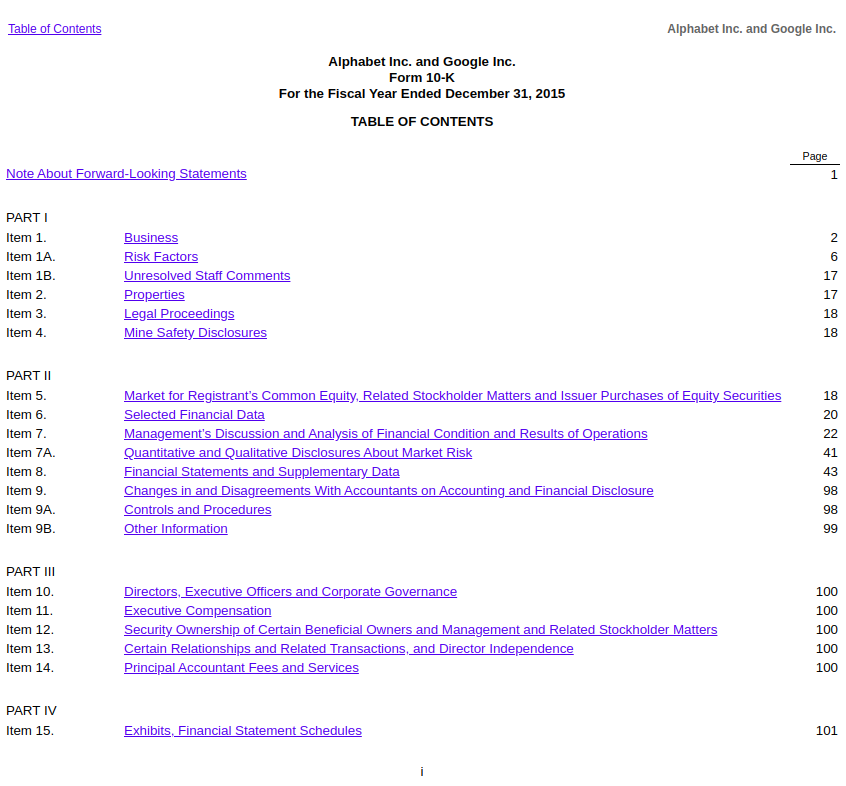
\includegraphics[scale=0.5]{toc.png}
\caption{SEC 10-K filing Table of Contents}
\end{figure}

As the project focuses on risks the only relevant section for it is assumed to be "Item 1A. Risk Factors" in which the risks and threats faced by business are discussed as well as the approaches to mitigating those risks.

\section{Related Research}
Emerging risk detection from SEC 10-K filings is not a well researched topic, however there exists some research on modelling constant, most common, reoccuring risks.

The most relevant and similar research has been done by Yang Bao and Anindya Datta (2012) \cite{riskpaper1}. They have built an algorithm based on latent Dirichlet allocation, which identifies the set of most common topics across the provided financial reports.

Most of previous work has been focused on tackling the risk detection task by using supervised methods, which proved to be fairly inefficient and unscalable. In this research, they built an unsupervised model based on latent Dirichlet allocation (LDA). 

The original LDA operates at the level of the words. However, as in the financial reports in most cases one sentence represents one risk topic, there may occur overlaps of topics in the sentences in case of original LDA. Therefore, they have developed sent-LDA, which tackles this problem by introducing sentence level calculations.

\begin{figure}[H]
\begin{center}
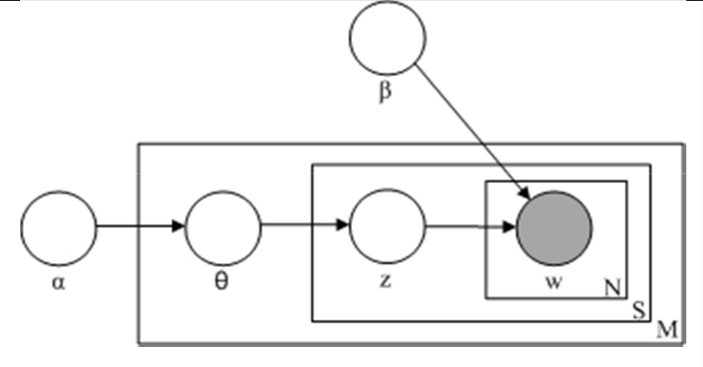
\includegraphics[scale=0.55]{sentLDA.png}
\caption{sent-LDA model representation \cite{riskpaper1}}
\end{center}
\end{figure}

The same notations are used as in original LDA (described in Section \ref{sec:lda}), introducing S as a sentence in a document. The model is created using the generative process (Figure \ref{fig:sentLDAgen}):

\begin{figure}[H]
\center
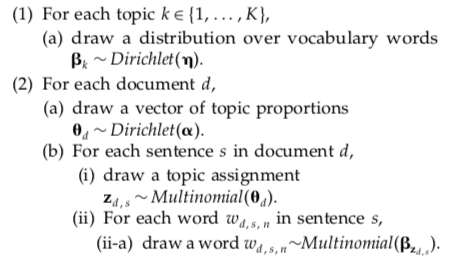
\includegraphics[scale=0.6]{sentLDApseudocode.png}
\caption{sent-LDA generative process \cite{riskpaper1}}
\label{fig:sentLDAgen}
\end{figure}

The described research has been a helpful starting point, which helped me understand the risk topic definitions, provided insight into constant reoccuring risks and helped define this projects approach to the task.
\\\\
Another research related to the project was done by S. Sehrawat \cite{10kwordembeddings}. In which he pre-trained word embeddings on SEC 10-K filings. The result of it was a 300-dimensional word embedding representation model.

\section{Constant Risks}
In this project the risks are categorized into known, constant risks - the risks that are reoccuring every year, such as \textit{catastrophes, financial liability and financing uncertainty} - and emerging risks - the risks that are novel and possibly unseen before, such as \textit{cybersecurity or COVID-19}. The constant risks are represented by a topic model, consisting of keywords and their frequencies. Risk topics are illustrated well by Yang Bao and Anindya Datta (2012) \cite{riskpaper1}:

\begin{figure}[H]
\center
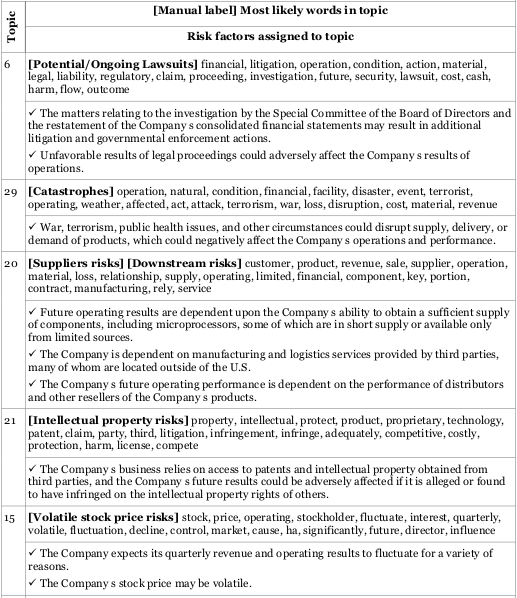
\includegraphics[scale=0.8]{risktopicfromriskpaper1.png}
\caption{Risk topic model example \cite{riskpaper1}}
\end{figure}

The constant risks and their topic model used in this project were generated in a research done by Dr. Stefan Petry\footnote{At the time of the writing the research is still ongoing, therefore the topics and their models cannot be publicly shared.}. The constant risk topic model contains 30 topics (constant risks), each defined by 30 keywords and their frequencies.